\documentclass[tikz,border=5mm]{standalone}
\usepackage{tikz}
\usetikzlibrary{arrows.meta, positioning, shapes.geometric, calc, patterns}

% --- COLOR DEFINITIONS ---
\definecolor{Garnet}{HTML}{73000A}
\definecolor{CBlue}{HTML}{466A9F}
\definecolor{CDark}{HTML}{1F414D}
\definecolor{CGold}{HTML}{A49137}
\definecolor{CGrayLight}{HTML}{E5E5E5}
\definecolor{CGrayDark}{HTML}{555555}
\definecolor{CWhite}{HTML}{FFFFFF}

\begin{document}

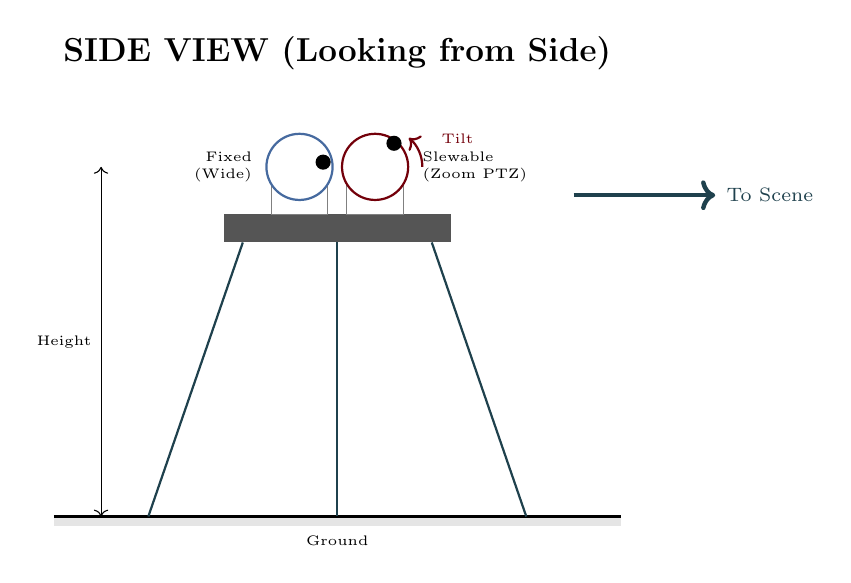
\begin{tikzpicture}[scale=1.2]
    % Title
    \node[font=\bfseries\large] at (0, 5) {SIDE VIEW (Looking from Side)};
    
    % Ground
    \fill[CGrayLight] (-3, 0) rectangle (3, 0.1);
    \draw[thick] (-3, 0.1) -- (3, 0.1);
    \node[below, font=\tiny] at (0, 0) {Ground};
    
    % Tripod Legs
    \draw[thick, CDark] (-1, 3) -- (-2, 0.1);
    \draw[thick, CDark] (1, 3) -- (2, 0.1);
    \draw[thick, CDark] (0, 3) -- (0, 0.1); % Center leg going back (appears as vertical)
    
    % Tripod Head / Mount Plate
    \fill[CGrayDark] (-1.2, 3) rectangle (1.2, 3.3);
    
    % Camera 1 (appears behind/left) - FIXED
    % In side view, both cameras appear stacked or overlapping since they are side-by-side
    % Show them slightly offset for clarity
    \begin{scope}[shift={(-0.4, 3.3)}]
        % Base
        \fill[CWhite] (-0.3, 0) rectangle (0.3, 0.5);
        \draw[gray] (-0.3, 0) rectangle (0.3, 0.5);
        % Dome
        \fill[CWhite] (0, 0.5) circle (0.35);
        \draw[CBlue, thick] (0, 0.5) circle (0.35);
        % Lens pointing forward (to the right in this view)
        \fill[black] (0.25, 0.55) circle (0.08);
        \node[left, font=\tiny, align=right] at (-0.4, 0.5) {Fixed\\(Wide)};
    \end{scope}
    
    % Camera 2 (appears in front/right) - SLEWABLE PTZ
    \begin{scope}[shift={(0.4, 3.3)}]
        % Base
        \fill[CWhite] (-0.3, 0) rectangle (0.3, 0.5);
        \draw[gray] (-0.3, 0) rectangle (0.3, 0.5);
        % Dome - tilted up
        \fill[CWhite] (0, 0.5) circle (0.35);
        \draw[Garnet, thick] (0, 0.5) circle (0.35);
        % Lens pointing up-right (tilted)
        \fill[black] (0.2, 0.75) circle (0.08);
        \node[right, font=\tiny, align=left] at (0.4, 0.5) {Slewable\\(Zoom PTZ)};
        
        % Tilt arrow
        \draw[->, Garnet, thick] (0.5, 0.5) arc (0:50:0.4);
        \node[right, font=\tiny, Garnet] at (0.6, 0.8) {Tilt};
    \end{scope}
    
    % Forward direction
    \draw[->, ultra thick, CDark] (2.5, 3.5) -- (4, 3.5) node[right, font=\scriptsize] {To Scene};
    
    % Height annotation
    \draw[<->, thin] (-2.5, 0.1) -- (-2.5, 3.8) node[midway, left, font=\tiny] {Height};
    
\end{tikzpicture}

\end{document}
